\documentclass[11pt,twoside,titlepage]{article}
\usepackage[english]{babel}
\usepackage{amsmath}
\usepackage{amsfonts}
\usepackage{graphicx}
\usepackage[font=small, format=hang]{caption}
\usepackage{hhline}
\usepackage{lineno}
\usepackage{fancyhdr}
\usepackage{calc}
\usepackage{url}
\usepackage{natbib}
\usepackage{color}
\usepackage{geometry}
\usepackage{epsfig}
\usepackage{endnotes}
\usepackage{upquote}
\usepackage{natbib}
\usepackage{mdwlist}
\usepackage{subcaption}
\usepackage{floatrow}
\renewcommand{\baselinestretch}{1.2}
\usepackage{geometry}
\geometry{ hmargin=2.5cm, vmargin=2.5cm }
\makeatletter
\def\iffloatpage#1#2{\if@fcolmade #1\else #2\fi}
\makeatother

\pagestyle{fancy}
%\fancyhead[LE,RO]{\iffloatpage{\thepage}{\thepage}}
%\fancyhead[RE]{\iffloatpage{}{{\small \textbf{\nouppercase \leftmark}}}}
%\fancyhead[LO]{\iffloatpage{}{\small \rightmark}}
%\renewcommand{\headrulewidth}{\iffloatpage{0pt}{0.4pt}}
\fancyhead[LE,RO]{\small{\textit{Seed Scientific\\Candidate Assignment 1}}}
\cfoot{\thepage}

\setlength{\headheight}{13.6pt}
\setlength{\marginparwidth}{0pt}
\setlength{\marginparsep}{0pt}
\setlength{\evensidemargin}{0pt}
\setlength{\oddsidemargin}{0pt}
%\renewcommand{\topmargin}{\iffloatpage{2pt}{22pt}}
%\renewcommand{\textwidth}{\iffloatpage{13cm}{360pt}}
\setlength{\hoffset}{\paperwidth/2-\textwidth/2-1in}


\renewcommand{\baselinestretch}{1.2}
\newcommand{\HRule}{\rule{\linewidth}{0.5mm}}
\def\dotsim{{\buildrel .\over \sim}}
\newcommand{\definition}{
\textbf{\textcolor{red}{Definition:}}
}
\renewcommand{\thefootnote}{\alph{footnote}}
\begin{document}
%\title{Automated Quality Assessment for Magnetic Resonance Images for Further Study in Alzeihmer's Disease Patients}
%\author{Marc Dupuis}
%\date{\today}
%\maketitle
%\begin{titlepage}
%\begin{center}
%
%{\textbf{Marc Dupuis\\}}
%\vspace*{0.2cm}
%\end{center}
%
%\pagenumbering{roman}
%\end{titlepage}
%\thispagestyle{empty}
\pagenumbering{roman}

\setcounter{page}{0}\pagenumbering{arabic}

%%	SMALL INTRODUCTION
\begin{titlepage}
\begin{center}

% Upper part of the page. The '~' is needed because \\
% only works if a paragraph has started.
\vspace*{4cm}
\Large Seed Scientific Candidate Assignment 1\\[0.5cm]

% Title

{ \huge \bfseries U.S.A. Passenger Airline Study}\\[0.4cm]

% Author and supervisor
Marc \textsc{Dupuis}\\
\small marc.f.dupuis@gmail.com\\
\small (980) 319-4717

\vfill

% Bottom of the page
{\large \today}

\end{center}
\end{titlepage}

\section{Project Specifications and Objectives}

The objective of this study is to investigate US passenger airline data using two datasets provided by Seed Scientific and the online Research and Innovative Technology Administration (RITA).

As stated in the prompt, the goal is to: \textit{demonstrate to Seed Scientific my ability to manage a real-world data set, to communicate and contextualize summary statistics, and, most importantly, my creativity and analytical rigor in generating and testing hypotheses.} Furthermore, it is explicitly stated that the assignment is deliberately unspecific and exploratory by nature.

\section{Introductory Note}

Seed Scientific provided two datasets as CSV files which held information on the carrier identification tags and airport locations. In addition to this, I was directed to the RITA website\footnote{http://www.transtats.bts.gov}, which holds data on US airline passenger flights. The available information is extremely diverse and rich, and contains data on departure dates, cities and airline as well as delays, cause of delays and cancellations.

The data from the RITA set is remarkably well organized and complete. There is no unexpected missing data and very little modifications had to be done in order to process the data.

\section{Results}

As an occasional passenger, the first questions that came to mind when I was given the data were: What do passenger flight trends look like? And what are the delay/cancellation trends? 

The number of US domestic flights is illustrated in Fig. \ref{fig:Number of Flights + Delays} for every month from January 2000 to August 2013. Two traits immediately stick out: a significant drop in flights around September 2001 and a sustained but progressive drop beginning in September 2008 (as marked by the red lines). These two dates match the 9/11 terrorist attacks and the US financial market crash of 2008 respectively. The 9/11 attacks caused a $22.72\%$ drop in flights from September to October 2001 and did not fully recover until a sudden surge around January 2003.

The blue lines mark other noticeable, yearly trends. There seems to be a surge in flights in summer and a drop around December (Christmas and New Year's eve). These trends were expected and are common knowledge.


Now that we've seen how the number of flights has evolved over the past 13 years, the next question is whether or not delays and cancellations have followed the same trends or if they have been increasing relative to the number of flights (I think we can all agree that it seems like every flight is delayed nowadays.) The most remarkable feature of cancellation and delay graphs is the ``insignificance'' of the number of cancelled flights relative to the total number of flights, as well as the sudden surge in cancellations around September 2001. Again, this surge marks the time of the 9/11 attacks. With regards to the delays, these seem to follow the same trends as the total number of flights. Given more time, several more advanced methods would do a better job confirming this, but the correlation between delayed flights and non-delayed flights is approximately $0.68$ versus $0.04$ for cancelled and on-time flights. This shows a rather strong correlation between number of flights and delays and a surprisingly low correlation between cancelled flights and other flights (including delayed flights).

\begin{figure}[h!]
        \centering
                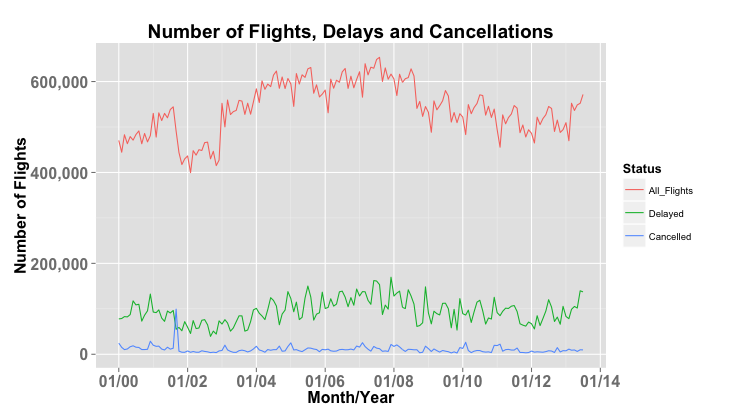
\includegraphics[width=17cm]{Number_of_Flights2.png}
        \caption{Flights, delays and cancellations from 2000 to 2013. The red lines indicate major events affecting the number of flights while the blue lines highlight yearly trends.}\label{fig:Number of Flights + Delays}
\end{figure}

Following the observations marked by the blue lines in Fig. \ref{fig:Number of Flights + Delays}, it would be interesting to look at the number of flights and delays by month (Fig. \ref{fig:Flights by Month}) The bar graph seems to support the idea of an increase of flights in the summer and a drop at the end of each year. However, the delays by month would be better expressed as a percentage of total flights. This is illustrated in Fig. \ref{fig:Flights by Month Percentage}. This bar graph seems to suggest that delays are rather steady with a slight increase around the summer period and Christmas holidays.

\begin{figure}[h!]
        \centering
                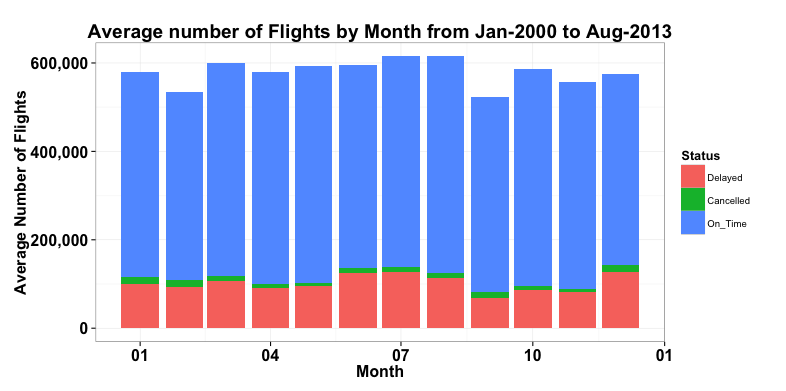
\includegraphics[width=16cm]{Bar1.png}
        \caption{Delays by month from January 2000 to August 2013.}\label{fig:Flights by Month}
\end{figure}

\begin{figure}[h!]
        \centering
                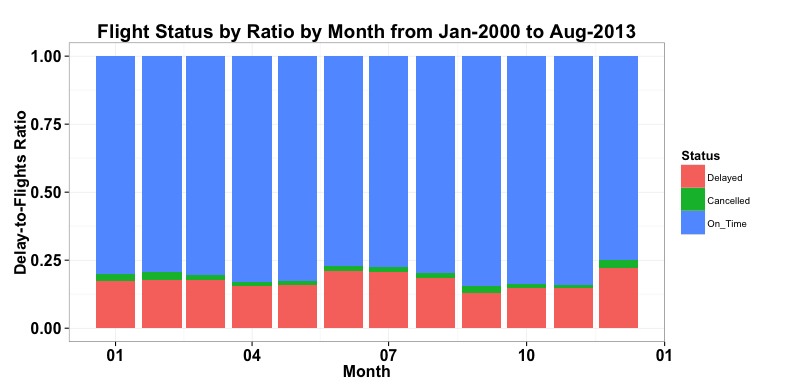
\includegraphics[width=16cm]{Bar2.png}
        \caption{Average number of flights by month expressed as a percentage of total flights each month.}\label{fig:Flights by Month Percentage}
\end{figure}

\clearpage
Now that we understand more about flight trends and delays/cancellations, it would be interesting to look at the causes of delays. Fig. \ref{fig:Pie} breaks up the causes of delays into five categories:
\begin{enumerate}\itemsep1pt \parskip0pt \parsep0pt
  \item Late aircraft
  \item National Airspace System (NAS) delay
  \item Carrier delay
  \item Weather
  \item Security
\end{enumerate}

With this figure however, it seems as if weather is not a frequent cause for delay, even though we would intuitively think that it is one of the main causes. This is because the NAS only categorizes delays as due to weather if the weather is severe\footnote{http://www.rita.dot.gov/bts/help/aviation/html/understanding.html}. Minor weather delays fall under NAS orders and thus contribute to the NAS section of the pie chart in addition to heavy air traffic and airport operations.

\begin{figure}[h!]
        \centering
                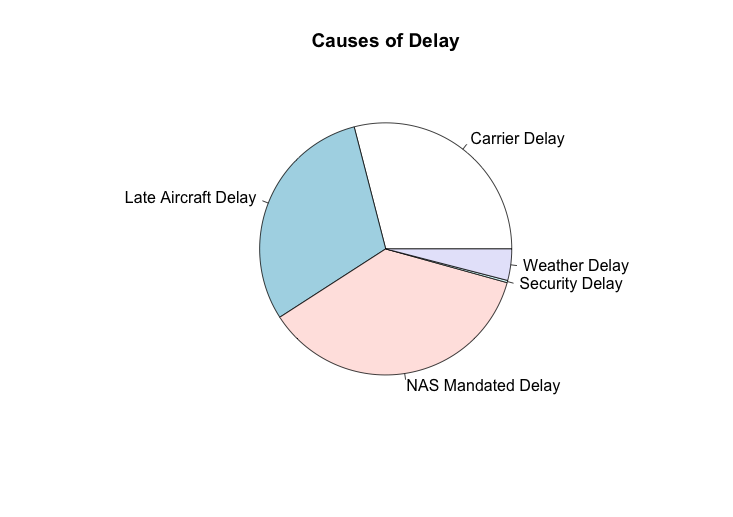
\includegraphics[width=16cm]{Pie.png}
        \caption{Pie chart illustrating main causes of US flight delays.}\label{fig:Pie}
\end{figure}

Now lets look at the delays by carrier relative to the total number of flights as illustrated in Fig. \ref{fig:Delays by Carrier as Percentage}. Atlantic Southeast Airlines, JetBlue and Southwest Airlines are the three worst performing airlines, while Hawaiian Airlines and Aloha Air Cargo are the best performing and perform exceptionally well.

\begin{figure}[h!]
        \centering
                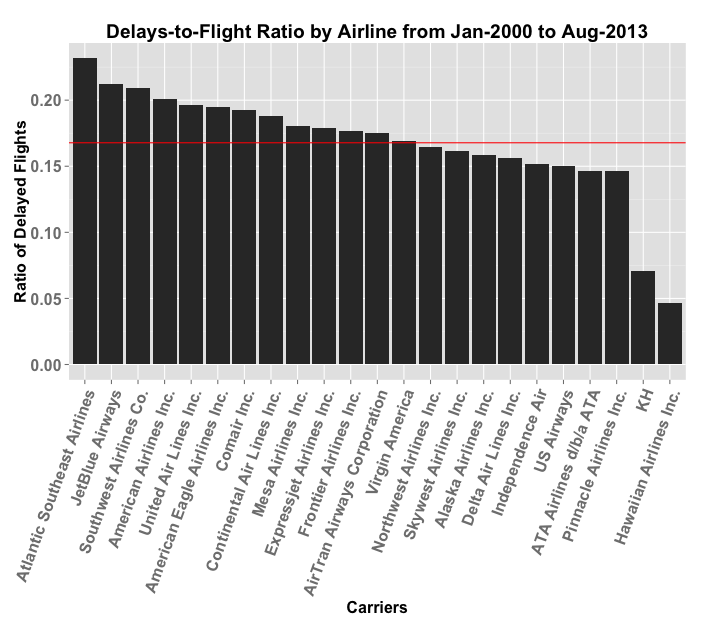
\includegraphics[width=16cm]{Delayed_by_Airline2.png}
        \caption{Delay-to-flight ratio by carrier. The red line indicates the mean of all ratios by carrier.}\label{fig:Delays by Carrier as Percentage}
\end{figure}

So we now know which airlines to avoid in terms of departure reliability and which to recommend. Lets now look at the relationship between delays and departure state. Fig. \ref{fig:Delays by State as Percentage} shows a fairly spread out distribution amongst all fifty states, Puerto Rico (PR), the Trusted Territories (TT) and the U.S. Virgin Islands (VI). As with the delays by carrier, we should look at this data relative to the number of flights departing from each of these states (Fig. \ref{fig:Delays by State as Percentage}). The best performers turn out to be Hawaii, Montana and Idaho. On the other hand, the worst performing states are the Trusted Territories, Illinois, New Jersey and Delaware (as illustrated in Fig. \ref{fig:USMap2}.) 

\begin{figure}[h!]
        \centering
                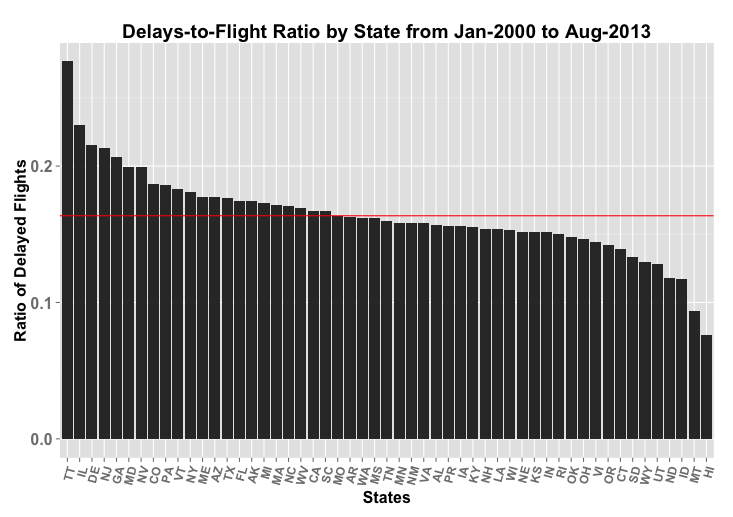
\includegraphics[width=17cm]{Delays_by_State2.png}
        \caption{Delay-to-flight ratio by state. The red line indicates the mean of all ratios by state.}\label{fig:Delays by State as Percentage}
\end{figure}

\begin{figure}[h!]
        \centering
                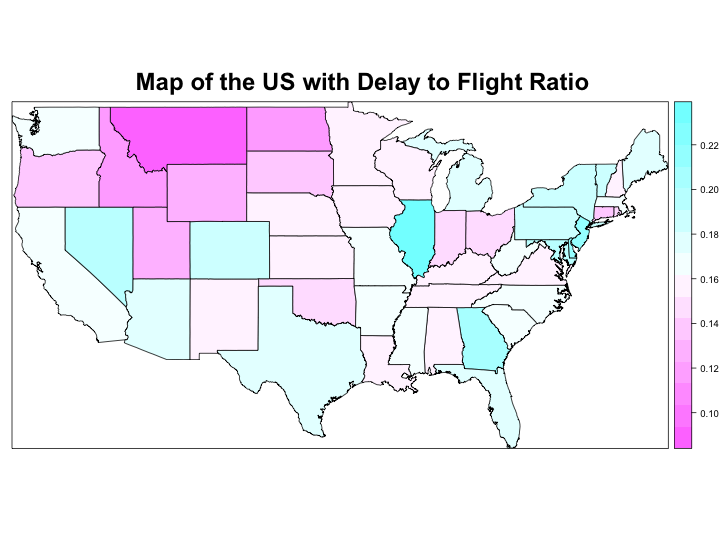
\includegraphics[width=14cm]{USMap2.png}
        \caption{Heatmap illustrating the delay-to-flight ratio for each state on the continent with Montana and Illinois on opposite ends of the spectrum.}\label{fig:USMap2}
\end{figure}

Finally, given the correlations that seems to exist between flight delay and carrier, month and departure state, if there is a significant connection between these features, a classifier should outperform random chance. Indeed, by applying a random forest, we can successfully determine whether or not a flight will be delayed with a $80.16\%$ success rate\footnote{Additional features used to the ones mentioned are arrival state and distance between departure and arrival states, and many more can and should be looked into. The classifier is also based on a significantly reduced dataset composed of $6.25\%$ of the available data due to limited memory availability.}; however, the Receiver Operator Characteristic (ROC) curve has an area of 0.607, which indicates that the classifier performs better than a random guess, but is not highly reliable.

\section{Conclusion}

There are several conclusions to draw from this investigation. First, as expected, customers flight patterns are affected by major disasters and the state of the economy. Preliminary indications seem to suggest that delays have not been increasing relative to the number of flights over the years and flight cancellations are relatively constant across time (aside from major disasters).

Second, delays are to be expected around the high traffic months during the summer as well as during the holiday season in December (we know how hard it can be to make it home for Christmas); however, the cause for delays is equally due to late aircrafts, carriers and NAS orders. It is difficult to truly assess the cause of a delay in the system. For instance, a late aircraft could be caused by weather in the state it came from or the carrier.

Finally, the scenario in which a passenger is least likely to experience any flight delay, is by travelling from Hawaii on Hawaiian Airlines in September\footnote{It's obviously not this straight forward as there are other important factors such as weather, human and natural disasters, day of the weak etc. And the delays should be considered by restricted geographical location.}. Similarly, a passenger is most likely to experience a delay if they travel at Christmas and they depart from Chicago with Southwest Airlines.

This study is very limited and is based on a number of assumptions which would have to be carefully considered in future investigations. The intent is to offer an initial perspective on flight patterns in the US and flight delay trends.

\clearpage
\break
\newpage

\section*{Appendix}
\vspace*{4cm}
\begin{figure}[h!]
        \centering
                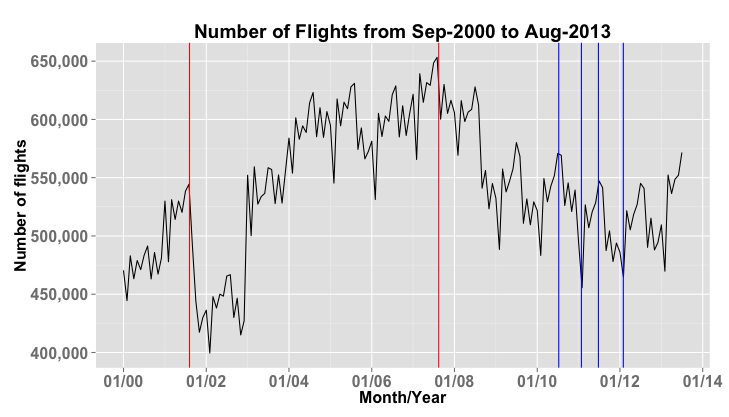
\includegraphics[width=15cm]{Number_of_Flights1.png}
        \caption{Number of US domestic flights from January 2000 to August 2013. The red lines indicate major events (9/11 terrorist attacks and beginning 2008 financial market crash after the subprime mortgage buble) and the blue lines indicate noticeable yearly trends.}\label{fig:Number of Flights}
\end{figure}


\begin{figure}[h!]
        \centering
                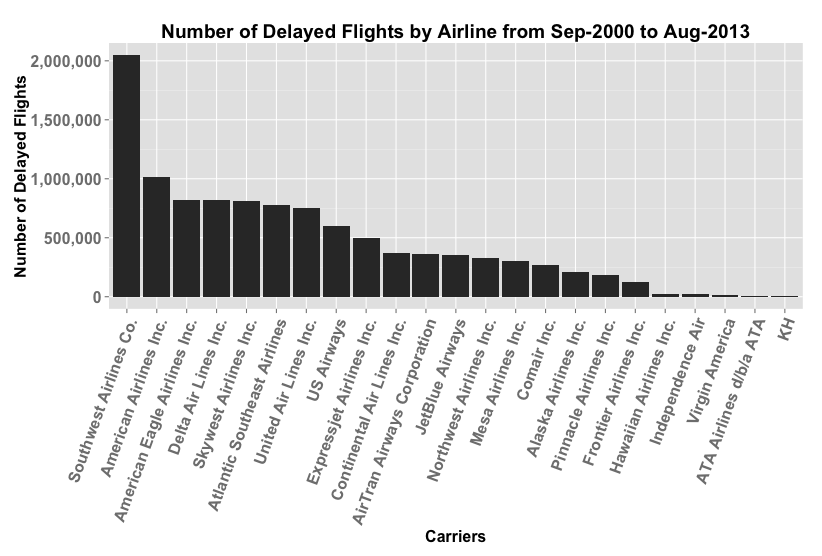
\includegraphics[width=16cm]{Delayed_by_Airline1.png}
        \caption{Total delays by carrier since January 2000. Southwest Airlines has over twice the amount as the second carrier ranked by number of delays.}\label{fig:Delays by Carrier}
\end{figure}

\begin{figure}[h!]
        \centering
                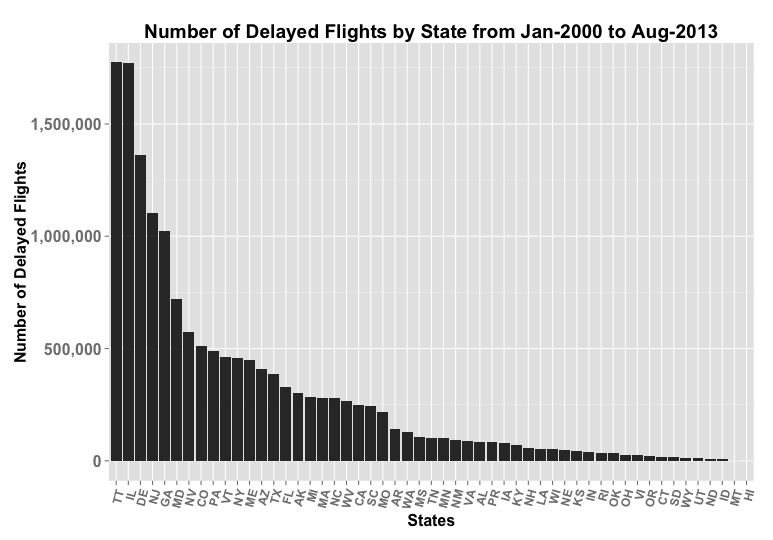
\includegraphics[width=16cm]{Delays_by_State1.png}
        \caption{Delays by departure state. The top six are somewhat expected: Texas, California, Illinois, Georgia, Florida and New York. These six states host six of the major airport hubs: Houston, Los Angeles (LAX), O'Hare, Atlanta, Miami and JFK.}\label{fig:Delays by State}
\end{figure}

\begin{figure}[h!]
        \centering
                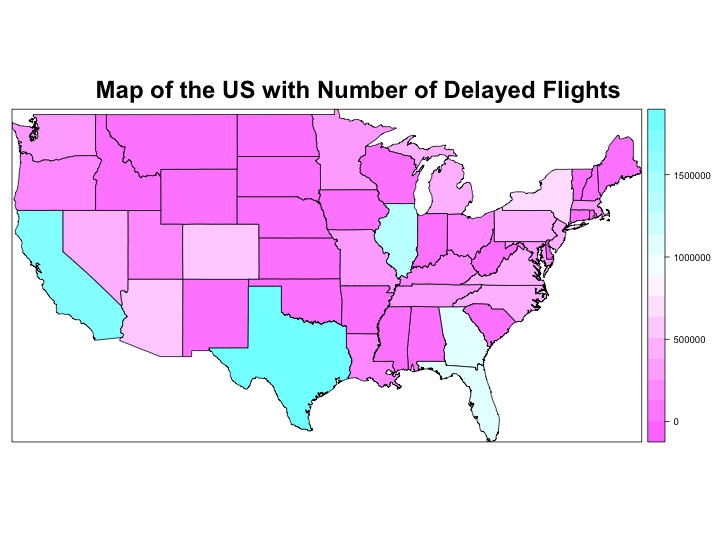
\includegraphics[width=16cm]{USMap1.png}
        \caption{Heatmap illustrating the number of delays by state since January 2000.}\label{fig:}
\end{figure}

\end{document}
